% The tkz-berge graph package
% Author: Alain Matthes (http://altermundus.fr/)

\documentclass[]{article}
\usepackage{tikz}
\usepackage{tikz,fullpage}
\usetikzlibrary{arrows,%
                petri,%
                topaths}%
\usepackage{tkz-berge}
\usepackage[position=top]{subfig}

\begin{document}

\iffalse
\begin{figure}
\centering
\subfloat[]{
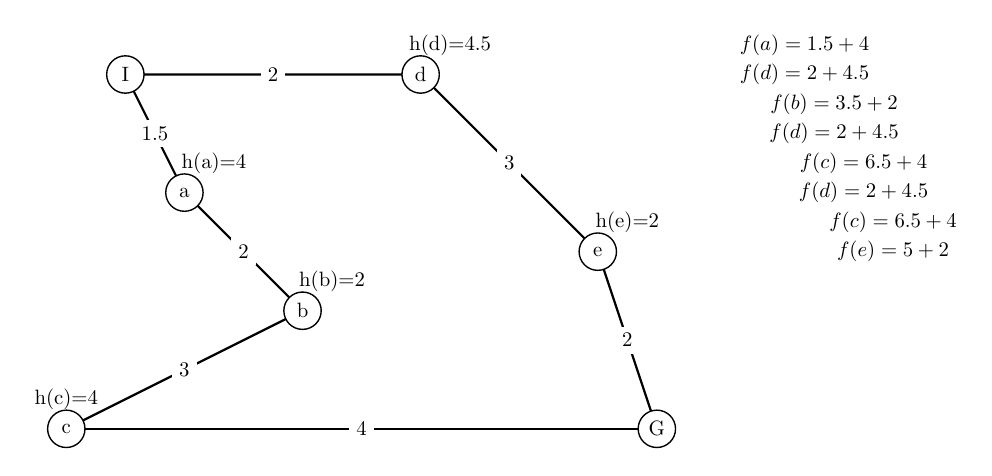
\begin{tikzpicture}[scale=0.75,transform shape]
  \Vertex[x=0,y=0]{c}
  \Vertex[x=4,y=2]{b}
  \Vertex[x=2,y=4]{a}
  \Vertex[x=1,y=6]{I}
  \Vertex[x=6,y=6]{d}
  \Vertex[x=9,y=3]{e}
  \Vertex[x=10,y=0]{G}
  %\tikzstyle{LabelStyle}=[fill=white,sloped]
  %\tikzstyle{EdgeStyle}=[bend left]
  \tikzstyle{EdgeStyle}=[]  
  \Edge[label=$2$](I)(d)
  \Edge[label=$1.5$](I)(a)
  \Edge[label=$2$](a)(b)
  \Edge[label=$3$](b)(c)
  \Edge[label=$4$](c)(G)
  \Edge[label=$3$](d)(e)
  \Edge[label=$2$](e)(G)
  
  \node [xshift=0cm,yshift=0.5cm] at (0,0) {h(c)=4};  
  \node [xshift=0.5cm,yshift=0.5cm] at (4,2) {h(b)=2};
  \node [xshift=0.5cm,yshift=0.5cm] at (2,4) {h(a)=4};
  \node [xshift=0.5cm,yshift=0.5cm] at (6,6) {h(d)=4.5};
  \node [xshift=0.5cm,yshift=0.5cm] at (9,3) {h(e)=2};
  
  \node [xshift=0.5cm,yshift=0.5cm] at (12,6) {$f(a) = 1.5 + 4$};  
  \node [xshift=0.5cm,yshift=0.5cm] at (12,5.5)  {$f(d) = 2 + 4.5$};   
  
  \node [xshift=1cm,yshift=0.5cm] at (12,5)  {$f(b) = 3.5 + 2$};
  \node [xshift=1cm,yshift=0.5cm] at (12,4.5)  {$f(d) = 2 + 4.5$};   
  
  \node [xshift=1.5cm,yshift=0.5cm] at (12,4)  {$f(c) = 6.5 + 4$};
  \node [xshift=1.5cm,yshift=0.5cm] at (12,3.5)  {$f(d) = 2 + 4.5$}; 
  
  \node [xshift=2cm,yshift=0.5cm] at (12,3)  {$f(c) = 6.5 + 4$};  
  \node [xshift=2cm,yshift=0.5cm] at (12,2.5)  {$f(e) = 5 + 2$};  
  
  
\end{tikzpicture}
}
\end{figure}



\begin{figure}
\centering
\subfloat[]{
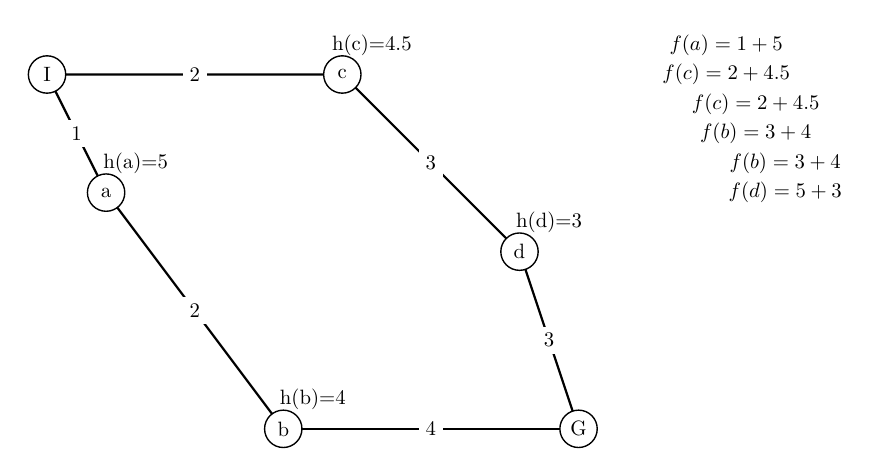
\begin{tikzpicture}[scale=0.75,transform shape]
  \Vertex[x=5,y=0]{b}
  \Vertex[x=2,y=4]{a}
  \Vertex[x=1,y=6]{I}
  \Vertex[x=6,y=6]{c}
  \Vertex[x=9,y=3]{d}
  \Vertex[x=10,y=0]{G}
  %\tikzstyle{LabelStyle}=[fill=white,sloped]
  %\tikzstyle{EdgeStyle}=[bend left]
  \tikzstyle{EdgeStyle}=[]  
  \Edge[label=$2$](I)(c)
  \Edge[label=$3$](c)(d)
  \Edge[label=$1$](I)(a)
  \Edge[label=$2$](a)(b)
  \Edge[label=$4$](b)(G)
  \Edge[label=$3$](d)(G)
  
  \node [xshift=0.5cm,yshift=0.5cm] at (5,0) {h(b)=4};  
  \node [xshift=0.5cm,yshift=0.5cm] at (2,4) {h(a)=5};
  \node [xshift=0.5cm,yshift=0.5cm] at (6,6) {h(c)=4.5};
  \node [xshift=0.5cm,yshift=0.5cm] at (9,3) {h(d)=3};
  
  \node [xshift=0.5cm,yshift=0.5cm] at (12,6) {$f(a) = 1 + 5$};  
  \node [xshift=0.5cm,yshift=0.5cm] at (12,5.5)  {$f(c) = 2 + 4.5$};   
  
  \node [xshift=1cm,yshift=0.5cm] at (12,5)  {$f(c) = 2 + 4.5$};
  \node [xshift=1cm,yshift=0.5cm] at (12,4.5)  {$f(b) = 3 + 4$};   
  
  \node [xshift=1.5cm,yshift=0.5cm] at (12,4)  {$f(b) = 3 + 4$};
  \node [xshift=1.5cm,yshift=0.5cm] at (12,3.5)  {$f(d) = 5 + 3$}; 

%  \node [xshift=2cm,yshift=0.5cm] at (12,3)  {$f(c) = 6.5 + 4$};  
%  \node [xshift=2cm,yshift=0.5cm] at (12,2.5)  {$f(e) = 5 + 2$};  
  
  
\end{tikzpicture}
}
\end{figure}


\begin{figure}
\centering
\subfloat[]{
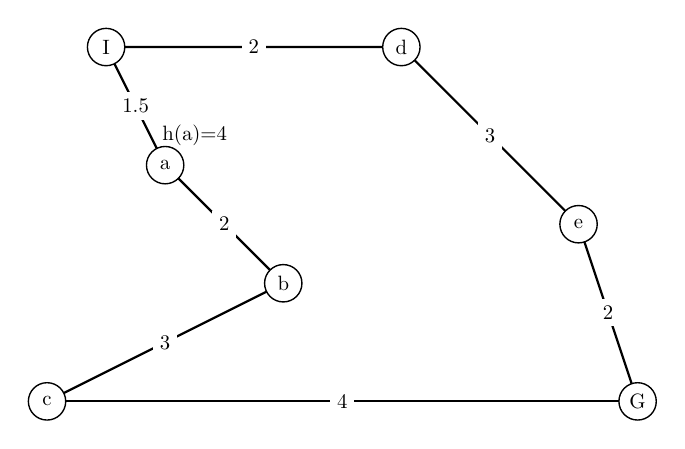
\begin{tikzpicture}[scale=0.75,transform shape]
  \Vertex[x=0,y=0]{c}
  \Vertex[x=4,y=2]{b}
  \Vertex[x=2,y=4]{a}
  \Vertex[x=1,y=6]{I}
  \Vertex[x=6,y=6]{d}
  \Vertex[x=9,y=3]{e}
  \Vertex[x=10,y=0]{G}
  %\tikzstyle{LabelStyle}=[fill=white,sloped]
  %\tikzstyle{EdgeStyle}=[bend left]
  \tikzstyle{EdgeStyle}=[]  
  \Edge[label=$2$](I)(d)
  \Edge[label=$1.5$](I)(a)
  \Edge[label=$2$](a)(b)
  \Edge[label=$3$](b)(c)
  \Edge[label=$4$](c)(G)
  \Edge[label=$3$](d)(e)
  \Edge[label=$2$](e)(G)
   
  \node [xshift=0.5cm,yshift=0.5cm] at (2,4) {h(a)=4};   
 
\end{tikzpicture}
}
%\end{figure}
%\begin{figure}
\centering
\subfloat[]{
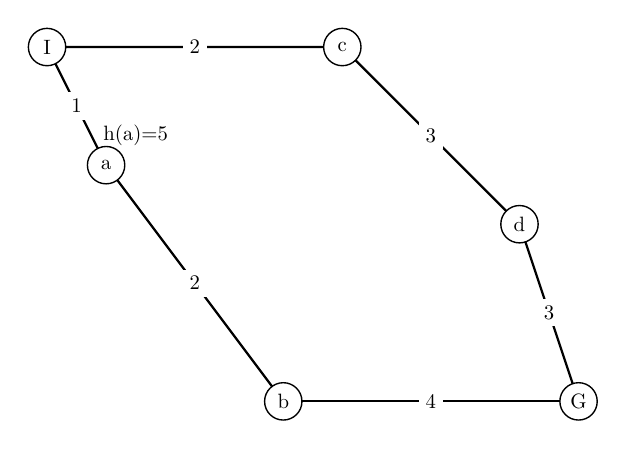
\begin{tikzpicture}[scale=0.75,transform shape]
  \Vertex[x=5,y=0]{b}
  \Vertex[x=2,y=4]{a}
  \Vertex[x=1,y=6]{I}
  \Vertex[x=6,y=6]{c}
  \Vertex[x=9,y=3]{d}
  \Vertex[x=10,y=0]{G}
  %\tikzstyle{LabelStyle}=[fill=white,sloped]
  %\tikzstyle{EdgeStyle}=[bend left]
  \tikzstyle{EdgeStyle}=[]  
  \Edge[label=$2$](I)(c)
  \Edge[label=$3$](c)(d)
  \Edge[label=$1$](I)(a)
  \Edge[label=$2$](a)(b)
  \Edge[label=$4$](b)(G)
  \Edge[label=$3$](d)(G)
  
  \node [xshift=0.5cm,yshift=0.5cm] at (2,4) {h(a)=5};  
  
\end{tikzpicture}
}
\end{figure}


\begin{figure}
\centering
\subfloat[]{
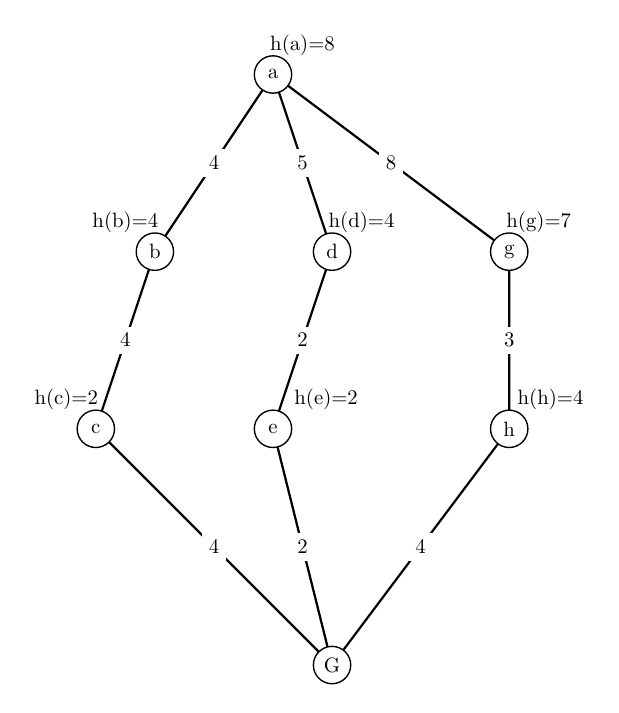
\begin{tikzpicture}[scale=0.75,transform shape]
  %\SetUpVertex[FillColor=blue!30]
  \Vertex[x=4,y=10]{a}
  \Vertex[x=2,y=7]{b}
  \Vertex[x=1,y=4]{c}
  \Vertex[x=5,y=7]{d}
  \Vertex[x=4,y=4]{e}
  \Vertex[x=5,y=0]{G}
  \Vertex[x=8,y=7]{g}
  \Vertex[x=8,y=4]{h}
  %\tikzstyle{LabelStyle}=[fill=white,sloped]
  %\tikzstyle{EdgeStyle}=[bend left]
  \tikzstyle{EdgeStyle}=[]  
  \Edge[label=$4$](a)(b)
  \Edge[label=$5$](a)(d)  
  \Edge[label=$8$](a)(g)
  \Edge[label=$4$](b)(c)
  \Edge[label=$4$](c)(G)
  \Edge[label=$2$](d)(e)
  \Edge[label=$2$](e)(G)
  \Edge[label=$3$](g)(h)
  \Edge[label=$4$](h)(G)   

  \node [xshift=0.5cm,yshift=0.5cm] at (4,10) {h(a)=8};  
  \node [xshift=-0.5cm,yshift=0.5cm] at (2,7) {h(b)=4};
  \node [xshift=-0.5cm,yshift=0.5cm] at (1,4) {h(c)=2};
  \node [xshift=0.5cm,yshift=0.5cm] at (5,7) {h(d)=4};
  \node [xshift=0.9cm,yshift=0.5cm] at (4,4) {h(e)=2};
  \node [xshift=0.5cm,yshift=0.5cm] at (8,7) {h(g)=7};
  \node [xshift=0.7cm,yshift=0.5cm] at (8,4) {h(h)=4};
   
  %\node [xshift=0.5cm,yshift=0.5cm] at (2,4) {h(a)=4};   
 
\end{tikzpicture}
}
\end{figure}
\fi


\begin{figure}
\centering
\subfloat[]{
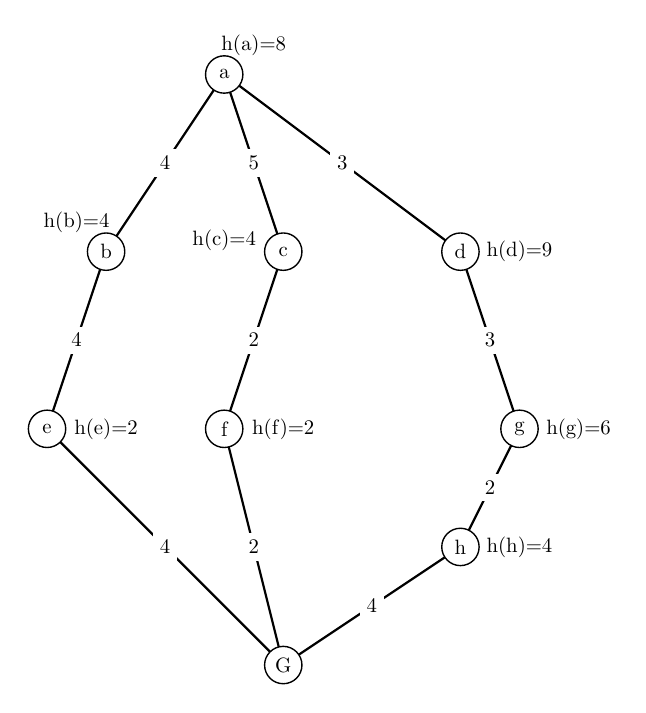
\begin{tikzpicture}[scale=0.75,transform shape]
  %\SetUpVertex[FillColor=blue!30]
  \Vertex[x=4,y=10]{a}
  \Vertex[x=2,y=7]{b}
  \Vertex[x=5,y=7]{c}  
  \Vertex[x=8,y=7]{d}
  \Vertex[x=1,y=4]{e}  
  \Vertex[x=4,y=4]{f}
  \Vertex[x=9,y=4]{g}
  \Vertex[x=8,y=2]{h}  
  \Vertex[x=5,y=0]{G}

  %\tikzstyle{LabelStyle}=[fill=white,sloped]
  %\tikzstyle{EdgeStyle}=[bend left]
  \tikzstyle{EdgeStyle}=[]
  \Edge[label=$4$](a)(b)
  \Edge[label=$5$](a)(c)
  \Edge[label=$3$](a)(d)
  \Edge[label=$4$](b)(e)
  \Edge[label=$4$](e)(G)
  \Edge[label=$2$](c)(f)
  \Edge[label=$2$](f)(G)
  \Edge[label=$3$](d)(g)
  \Edge[label=$2$](g)(h)
  \Edge[label=$4$](h)(G)

  \node [xshift=0.5cm,yshift=0.5cm] at (4,10) {h(a)=8};
  \node [xshift=-0.5cm,yshift=0.5cm] at (2,7) {h(b)=4};
  \node [xshift=-1cm,yshift=0.2cm] at (5,7) {h(c)=4};
  \node [xshift=1cm,yshift=0cm] at (8,7) {h(d)=9};
  \node [xshift=1.0cm,yshift=0cm] at (1,4) {h(e)=2};
  \node [xshift=1cm,yshift=0cm] at (4,4) {h(f)=2};
  \node [xshift=1cm,yshift=0cm] at (9,4) {h(g)=6};
  \node [xshift=1cm,yshift=0cm] at (8,2) {h(h)=4};

\end{tikzpicture}
}
\end{figure}



\begin{figure}
\centering
\subfloat[]{
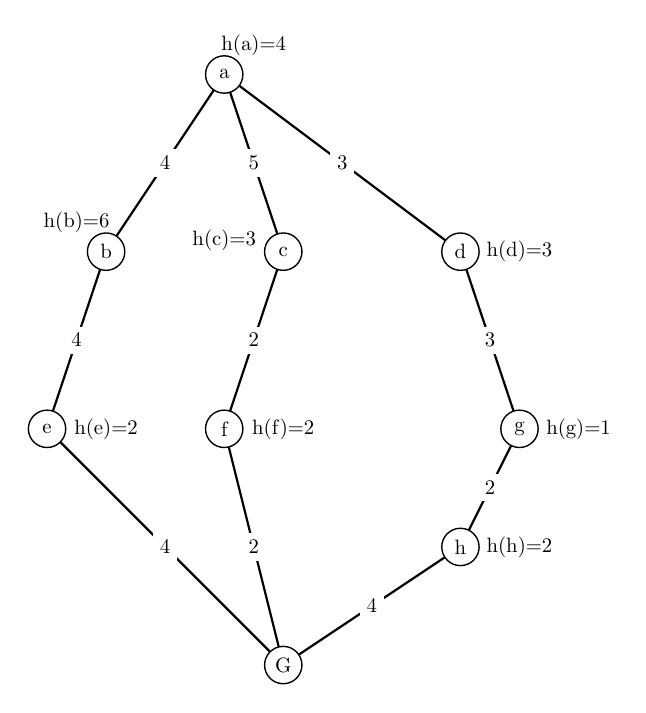
\begin{tikzpicture}[scale=0.75,transform shape]
  %\SetUpVertex[FillColor=blue!30]

  \Vertex[x=4,y=10]{a}
  \Vertex[x=2,y=7]{b}
  \Vertex[x=5,y=7]{c}  
  \Vertex[x=8,y=7]{d}
  \Vertex[x=1,y=4]{e}  
  \Vertex[x=4,y=4]{f}
  \Vertex[x=9,y=4]{g}
  \Vertex[x=8,y=2]{h}  
  \Vertex[x=5,y=0]{G}

  \tikzstyle{EdgeStyle}=[]
  \Edge[label=$4$](a)(b)
  \Edge[label=$5$](a)(c)
  \Edge[label=$3$](a)(d)
  \Edge[label=$4$](b)(e)
  \Edge[label=$4$](e)(G)
  \Edge[label=$2$](c)(f)
  \Edge[label=$2$](f)(G)
  \Edge[label=$3$](d)(g)
  \Edge[label=$2$](g)(h)
  \Edge[label=$4$](h)(G)
  
  \node [xshift=0.5cm,yshift=0.5cm] at (4,10) {h(a)=4};
  \node [xshift=-0.5cm,yshift=0.5cm] at (2,7) {h(b)=6};
  \node [xshift=-1cm,yshift=0.2cm] at (5,7) {h(c)=3};
  \node [xshift=1cm,yshift=0cm] at (8,7) {h(d)=3};
  \node [xshift=1.0cm,yshift=0cm] at (1,4) {h(e)=2};
  \node [xshift=1cm,yshift=0cm] at (4,4) {h(f)=2};
  \node [xshift=1cm,yshift=0cm] at (9,4) {h(g)=1};
  \node [xshift=1cm,yshift=0cm] at (8,2) {h(h)=2};

\end{tikzpicture}
}
\end{figure}




\begin{figure}
\centering
\subfloat[]{
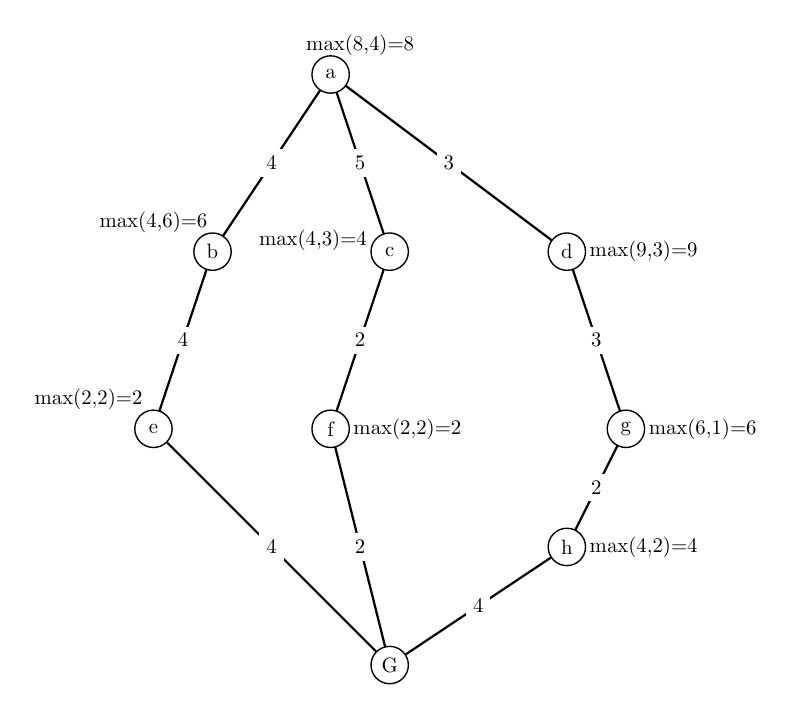
\begin{tikzpicture}[scale=0.75,transform shape]
  \Vertex[x=4,y=10]{a}
  \Vertex[x=2,y=7]{b}
  \Vertex[x=5,y=7]{c}  
  \Vertex[x=8,y=7]{d}
  \Vertex[x=1,y=4]{e}  
  \Vertex[x=4,y=4]{f}
  \Vertex[x=9,y=4]{g}
  \Vertex[x=8,y=2]{h}  
  \Vertex[x=5,y=0]{G}

  \tikzstyle{EdgeStyle}=[]
  \Edge[label=$4$](a)(b)
  \Edge[label=$5$](a)(c)
  \Edge[label=$3$](a)(d)
  \Edge[label=$4$](b)(e)
  \Edge[label=$4$](e)(G)
  \Edge[label=$2$](c)(f)
  \Edge[label=$2$](f)(G)
  \Edge[label=$3$](d)(g)
  \Edge[label=$2$](g)(h)
  \Edge[label=$4$](h)(G)


  \node [xshift=0.5cm,yshift=0.5cm] at (4,10) {max(8,4)=8};
  \node [xshift=-1cm,yshift=0.5cm] at (2,7) {max(4,6)=6};
  \node [xshift=-1.3cm,yshift=0.2cm] at (5,7) {max(4,3)=4};
  \node [xshift=1.3cm,yshift=0cm] at (8,7) {max(9,3)=9};
  \node [xshift=-1.1cm,yshift=0.5cm] at (1,4) {max(2,2)=2};
  \node [xshift=1.3cm,yshift=0cm] at (4,4) {max(2,2)=2};
  \node [xshift=1.3cm,yshift=0cm] at (9,4) {max(6,1)=6};
  \node [xshift=1.3cm,yshift=0cm] at (8,2) {max(4,2)=4};






\end{tikzpicture}
}
\end{figure}

\end{document}